%==============================================================================
% Supplement to "Feature-Aligned Adaptive Triggers ..." (FAAT)
% Standalone doc. Compile: latexmk -pdf supplement
%==============================================================================
\documentclass[10pt,twocolumn,letterpaper]{article}
\usepackage{cvpr}
%% Additional packages and macros for the FAAT paper.
%% Loaded by main.tex before hyperref.

% --- pseudo-code ---
\usepackage{algorithm}
\usepackage{algorithmic}

% (architecture diagram F2 is rendered with matplotlib -> no tikz needed;
%  tikz pulls everyshi which clashes with cvpr.sty's inlined everyshi.)
\floatname{algorithm}{Algorithm}
\renewcommand{\algorithmicrequire}{\textbf{Input:}}
\renewcommand{\algorithmicensure}{\textbf{Output:}}

% --- tables / layout ---
\usepackage{multirow}
\usepackage{array}
\usepackage{cuted}     % strip environment (two-column teaser)
\usepackage{currfile}  % \currfilebase

% --- inline annotations (disable for final) ---
\newcommand{\red}[1]{{\color{red}#1}}
\newcommand{\todo}[1]{{\color{red}#1}}
\newcommand{\TODO}[1]{\textbf{\color{red}[TODO: #1]}}
% For camera-ready, uncomment to hide todos:
% \renewcommand{\TODO}[1]{}
% \renewcommand{\todo}[1]{#1}

% --- paper-specific macros ---
\newcommand{\faat}{FAAT}                         % our main method
\newcommand{\kst}{KST}                           % spectrum-flat trigger
\newcommand{\sdt}{SDT}                           % Stein trigger
\newcommand{\dglobal}{\delta_{\mathrm{g}}}       % global trigger
\newcommand{\dadapt}{\delta_{\mathrm{a}}}        % adaptive residual
\newcommand{\Lalign}{\mathcal{L}_{\mathrm{align}}}
\newcommand{\asr}{\mathrm{ASR}}                  % attack success rate
\newcommand{\ba}{\mathrm{BA}}                    % benign accuracy
\newcommand{\ours}{\textbf{Ours}}                % bold "Ours" in tables
\newcommand{\na}{\textendash}                    % placeholder for not-yet-filled cells
\newcommand{\secsub}[1]{\textsubscript{#1}}      % tiny subscript helper

\definecolor{cvprblue}{rgb}{0.21,0.49,0.74}
\usepackage[breaklinks,colorlinks,allcolors=cvprblue]{hyperref}
\def\confName{CVPR}\def\confYear{2026}

\title{Supplementary Material:\\
Feature-Aligned Adaptive Triggers for Effective and Stealthy\\
Clean-Label Backdoor Attacks}
\author{Anonymous Author(s)}

\begin{document}
\maketitle

\section{Per-dataset FAAT detail}
\label{sec:faat-detail}
Table~\ref{tab:faat-detail} gives FAAT's full per-$\ell_2$, 3-seed results
(ASR mean$\pm$std). All values are end-of-training (last-20-epoch) means.
GTSRB uses a larger budget because of its $43$-class, BA$\approx\!100\%$ regime.

\begin{table}[h]
\centering
\small
\setlength{\tabcolsep}{3.5pt}
\begin{tabular}{l c c c c c c}
\toprule
Dataset (rate) & $\ell_2$ & ASR & $\sigma_{\asr}$ & BA & SSIM & SS$^\star$ \\
\midrule
CIFAR-10 (1\%)   & 0.9 & 76.1 & 2.5 & 94.8 & 0.981 & 0.438 \\
                 & 1.2 & 88.6 & 0.9 & 94.7 & 0.967 & 0.455 \\
                 & 1.5 & 93.6 & 1.9 & 94.8 & 0.950 & 0.433 \\
\midrule
GTSRB (1\%)      & 2.5 & 64.5 & 3.4 & 99.9 & 0.805 & 0.790 \\
                 & 3.0 & 71.5 & 1.8 & 99.9 & 0.761 & 0.733 \\
                 & 3.5 & 82.7 & 2.7 & 99.8 & 0.720 & 0.737 \\
\midrule
CIFAR-100 (1\%)  & 1.5 & 99.1 & 0.1 & 77.1 & 0.949 & 0.208 \\
                 & 2.0 & 99.6 & 0.1 & 77.3 & 0.919 & 0.200 \\
                 & 2.5 & 99.6 & 0.1 & 77.0 & 0.888 & 0.212 \\
\midrule
CIFAR-100 (0.5\%)& 1.5 & 96.8 & 0.6 & 77.9 & 0.949 & 0.262 \\
                 & 2.0 & 98.5 & 0.6 & 77.6 & 0.919 & 0.246 \\
                 & 2.5 & 99.4 & 0.2 & 77.9 & 0.888 & 0.236 \\
\midrule
Tiny-IN (0.25\%) & 1.5 & 93.0 & 2.0 & 55.0 & 0.952 & 0.265 \\
                 & 2.0 & 95.8 & 1.3 & 54.7 & 0.927 & 0.249 \\
                 & 2.5 & 94.8 & 0.9 & 54.5 & 0.902 & 0.248 \\
\bottomrule
\end{tabular}
\caption{FAAT per-$\ell_2$ detail (3 seeds). $^\star$SS-AUC reported as
$1{-}$AUC (lower = more evasive). Source: \texttt{docs/\{v4,v6,v6c,v7\}\_results.json}.}
\label{tab:faat-detail}
\end{table}

\section{Defense detail (selection $\times$ defense)}
\label{sec:defense-detail}
Table~\ref{tab:defense-detail} reports post-defense ASR and benign accuracy for
the Component-A (res$_x^2$) vs.\ random selection on the baseline authors'
defense benchmark. The strongest model-repair defenses (ABL, RNP) reduce ASR but
also collapse benign accuracy (RNP: $\ba\!\downarrow$ to $44$), limiting their
practical use.

\begin{table}[h]
\centering
\small
\setlength{\tabcolsep}{4pt}
\begin{tabular}{l c c c c}
\toprule
& \multicolumn{2}{c}{res$_x^2$ (ours)} & \multicolumn{2}{c}{random} \\
\cmidrule(lr){2-3}\cmidrule(lr){4-5}
Defense & ASR$\downarrow$ & BA & ASR$\downarrow$ & BA \\
\midrule
AC~\cite{chen2018activation}    & 75.1 & 89.2 & 55.2 & 89.7 \\
NC~\cite{wang2019neuralcleanse} & 75.5 & 92.5 & 42.9 & 93.0 \\
FST                             & 76.6 & 91.8 & 54.0 & 92.5 \\
FP~\cite{liu2018finepruning}    & 66.4 & 92.2 & 50.6 & 92.4 \\
ABL~\cite{li2021abl}            & 21.8 & 62.1 & 19.2 & 61.1 \\
RNP~\cite{lyu2023rnp}           & 24.8 & 44.1 & 12.6 & 51.3 \\
I-BAU~\cite{zeng2021ibau}       & 23.1 & 87.9 & 21.4 & 88.6 \\
\bottomrule
\end{tabular}
\caption{Post-defense ASR (\%) and BA (\%) by selection. Source:
\texttt{defense\_results/summary.csv} (authors' logs).}
\label{tab:defense-detail}
\end{table}

\section{KST multi-dataset campaign}
\label{sec:kst-campaign}
Table~\ref{tab:kst-campaign} reports KST at the operating $\varepsilon\!=\!48/255$
on the harder datasets (where the flat-spectrum trigger becomes learnable);
lower $\varepsilon$ and GTSRB are pending (\na).

\begin{table}[h]
\centering
\small
\begin{tabular}{l c c c c}
\toprule
Dataset (rate) & $\varepsilon$ & selection & ASR & BA \\
\midrule
CIFAR-100 (0.5\%) & 48 & forget    & 83.3 & 78.1 \\
                  & 48 & res$_x$   & \textbf{93.9} & 78.0 \\
Tiny-IN (0.25\%)  & 48 & forget    & 98.5 & 55.4 \\
                  & 48 & res$_x$   & \textbf{98.5} & 55.2 \\
GTSRB (1\%)       & 20 & forget / res$_x$ & 0.0 & 100.0 \\
                  & 48 & forget    & 0.8$^\dagger$ & 100.0 \\
\bottomrule
\end{tabular}
\caption{KST multi-dataset. $^\dagger$peak $19.3\%$ at epoch 139 then collapse
to $0.8\%$ (Fig.~\ref{fig:gtsrb-dyn}). On GTSRB KST stays stealthy (SSIM $0.94$
at $\varepsilon\!=\!20$) but fails to flip the overconfident victim. Sources:
\texttt{results/kst\_sdt/c100\_kst\_e48\_*/output\_1.log},
\texttt{tiny\_kst\_e48\_*/output\_1.log},
\texttt{gtsrb\_kst\_e48\_forget/output\_1.log}.}
\label{tab:kst-campaign}
\end{table}

\section{Reproduced CIFAR-10 Table-1}
\label{sec:baseline-table1}
Table~\ref{tab:baseline-table1} is our full reproduction of the clean-label
components' Table-1 (4 attacks $\times$ 8 selections, ASR last-20-epoch mean),
confirming the selection ranking (res$_x$ and res$_x^2$ dominate) used to choose
Component-A.

\begin{table}[h]
\centering
\small
\setlength{\tabcolsep}{3.2pt}
\begin{tabular}{l c c c c}
\toprule
selection & BadNets-C & Blended-C & MultiBpp-RGB & MultiBpp-B \\
\midrule
random    & 37.2 & 53.4 & 1.2  & 1.4  \\
loss      & 52.7 & 59.4 & 47.9 & 28.0 \\
gradient  & 52.6 & 60.2 & 53.3 & 38.3 \\
forget    & 71.7 & 71.1 & 78.1 & 81.0 \\
res-log   & 75.9 & 82.3 & 82.1 & 89.7 \\
res-x     & 68.8 & 82.3 & 85.1 & 89.7 \\
res-x$^2$ & 70.6 & 75.9 & 82.5 & 85.4 \\
res-e$^x$ & 66.7 & 71.8 & 62.3 & 53.9 \\
\bottomrule
\end{tabular}
\caption{Reproduced CIFAR-10 ASR (\%), 1\% poison, 300 epochs. Source:
\texttt{results/\_detail\_summary.json}.}
\label{tab:baseline-table1}
\end{table}

\begin{figure}[t]
\centering
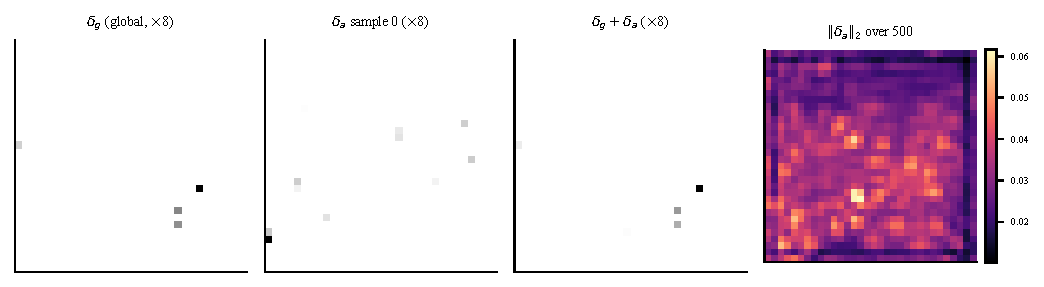
\includegraphics[width=\linewidth]{floats/figures/f9_trigger_viz.pdf}
\caption{\textbf{FAAT trigger visualization} (CIFAR-10). Global $\dglobal$, a
sample adaptive residual $\dadapt^{(0)}$, their sum (all amplified $\times$8), and
the average $\ell_2$-norm map of $\dadapt$ across $500$ poisoned samples.}
\label{fig:trig}
\end{figure}


\section{Additional visualizations}
\begin{figure}[h]
\centering
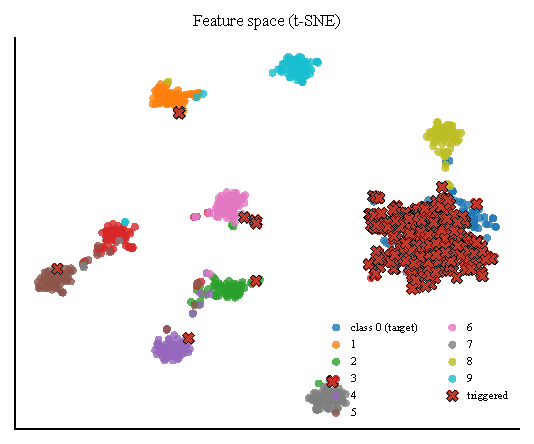
\includegraphics[width=0.92\linewidth]{floats/figures/f10_tsne.pdf}
\caption{\textbf{Feature-space t-SNE} of the FAAT victim (CIFAR-10). Each class
is a color; red $\times$ are non-target test images with the test trigger
applied. Triggered images migrate into the target-class (class 0) cluster,
confirming the global direction is a strong backdoor signal in feature space.}
\label{fig:tsne}
\end{figure}

\begin{figure}[h]
\centering
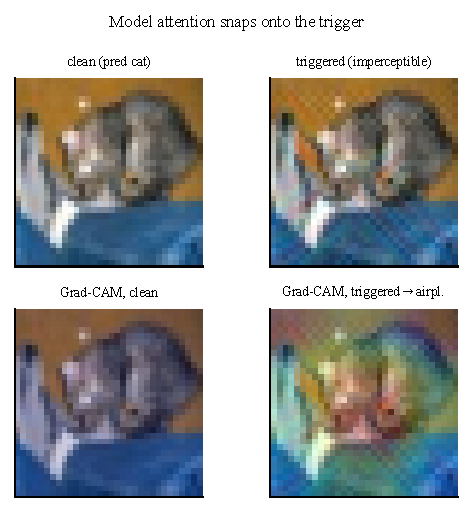
\includegraphics[width=0.8\linewidth]{floats/figures/f11_gradcam.pdf}
\caption{\textbf{Grad-CAM on the target logit} (CIFAR-10). On a clean cat image
the model attends normally; after the imperceptible trigger the attention snaps
onto the trigger and the prediction flips to the target class.}
\label{fig:gradcam}
\end{figure}

\begin{figure*}[t]
\centering
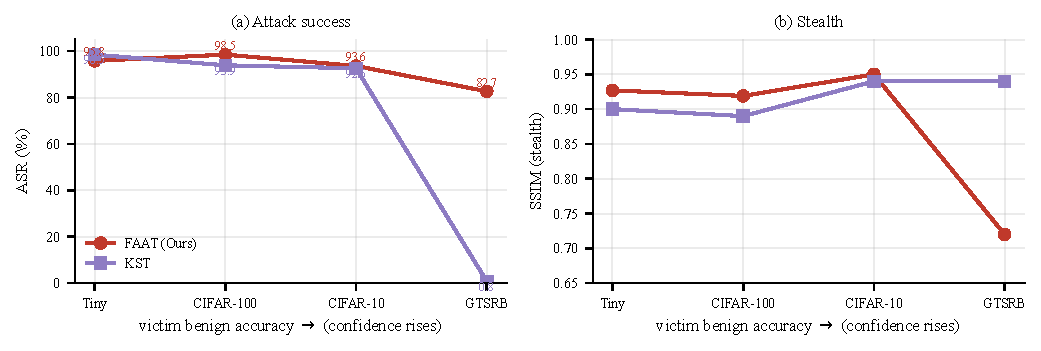
\includegraphics[width=0.92\linewidth]{floats/figures/f13_confidence_axis.pdf}
\caption{\textbf{The ASR--stealth window narrows with victim confidence.} Moving
right (Tiny $\to$ CIFAR-100 $\to$ CIFAR-10 $\to$ GTSRB, by rising benign
accuracy), FAAT holds ASR but loses stealth on GTSRB, while KST holds stealth
but loses ASR. No method keeps both at the high-confidence end.}
\label{fig:conf-axis}
\end{figure*}

Physical-robustness curves (JPEG/rotation/scaling) are generated from the same
trained models and will be inserted here (\na).

{\small
\bibliographystyle{ieeenat_fullname}
\bibliography{refs}
}

\end{document}
